\begin{tabular}{l|c}
Rollen S. D'Souza is currently a PhD Candidate in Electrical \& Computer Engineering specializing in the theory of nonlinear control design at the \href{https://uwaterloo.ca/}{University of Waterloo} in Waterloo, Ontario, Canada.
He is supervised by \href{https://ece.uwaterloo.ca/~cnielsen/}{Prof. Chris Nielsen}.
&
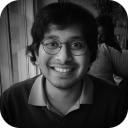
\includegraphics{images/rollen-128.png}
\end{tabular}
\paragraph{Recent Posts}
\begin{itemize}
  $partial("templates/post-list.tex")$
\end{itemize}

\paragraph{More About Rollen}
Rollen graduated in 2017 with his Bachelors of Software Engineering (B.S.E.) during which he completed a number of cooperative work terms in the software engineering field with applications in game development, media programming and application programming.
He complimented his degree with a joint in Applied Mathematics.
Late in the degree, his interests drove towards the general mathematics of control theory and its applications to robotics and aerospace.

Currently Rollen investigates an application of \href{https://en.wikipedia.org/wiki/Differential_ideal}{exterior differential systems} to solving \href{https://en.wikipedia.org/wiki/Feedback_linearization}{feedback equivalence problems}.
These are problems that appear in designing nonlinear control laws for nonlinear systems such as those that model the physical (Newtonian) dynamics of a robotic arm.
